\documentclass[12pt,a4paper]{article}
\usepackage[utf8]{inputenc}
\usepackage{graphicx}
\usepackage{float}
\usepackage{amsmath}
\usepackage{listings}
\usepackage{hyperref}
\usepackage{geometry}
\usepackage{subcaption}

\geometry{
  a4paper,
  total={170mm,257mm},
  left=20mm,
  top=20mm,
}
\hypersetup{
  colorlinks=false, % Disable colored text
  pdfborder={0 0 0} % Remove border around links
}

\graphicspath{{output/}}

\title{Image And Video Processing Lab Experiments}
\author{Vishal Murugan DBS}
\date{}
\begin{document}

\maketitle
\tableofcontents
\newpage

\section*{Experiment Number: 1}
\section {Eye Detection using Haar Cascade Classifiers}

\subsection{Brief Description about the Theory}
This experiment demonstrates the implementation of face and eye detection using Haar Cascade Classifiers. The system uses OpenCV's pre-trained cascade classifiers to detect faces and eyes in images or real-time video streams. The Haar cascade algorithm is based on machine learning and is trained with positive and negative images to recognize specific features.

\subsection{Experimental Details}
\subsubsection{Implementation Details}
\begin{itemize}
  \item Uses Haar Cascade Classifiers for face and eye detection.
  \item Converts input image to grayscale for processing.
  \item Implements both image and video processing capabilities.
  \item Draws circles around detected eyes for visualization.
\end{itemize}

\subsubsection{Technical Approach}
The implementation follows these key steps:
\begin{enumerate}
  \item Image Pre-processing:
    \begin{itemize}
      \item Converts the input image to grayscale for efficient processing.
      \item Uses pre-trained Haar cascade classifiers for face and eye detection.
    \end{itemize}

  \item Face Detection:
    \begin{itemize}
      \item Applies the face cascade classifier with scale factor 1.3 and minimum neighbors 4.
      \item Creates regions of interest (ROI) for each detected face.
    \end{itemize}

  \item Eye Detection:
    \begin{itemize}
      \item Processes each face ROI separately for eye detection.
      \item Calculates eye center and radius for visualization.
      \item Draws red circles (RGB: 0,0,255) around detected eyes.
    \end{itemize}
\end{enumerate}

\subsection{Results and Inferences}
The system successfully detected faces and eyes in both image and video streams. The implementation of Haar Cascade Classifiers proved effective in real-time detection. However, detection accuracy is influenced by lighting conditions and image resolution. Future improvements may include deep learning-based approaches for enhanced accuracy.

\begin{figure}[H]
  \centering
  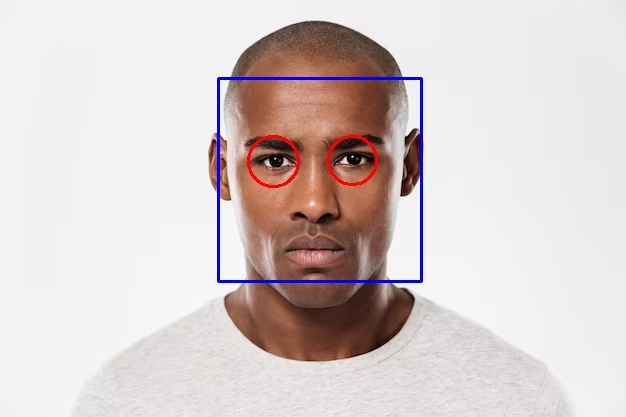
\includegraphics[width=0.7\textwidth]{eye_detection/eye_detection_result.jpg}
  \caption{Eye Detection Results}
  \label{fig:eye_detection}
\end{figure}

\newpage
\section*{Experiment Number: 2}
\section{Image Transformation Techniques}

\subsection{Brief Description about the Theory}
Image transformations are fundamental operations that modify the spatial arrangement or color representation of pixels. These transformations are widely used in computer vision for preprocessing, feature extraction, and data augmentation.

\subsection{Experimental Details}
\subsubsection{Geometric Transformations}
\begin{itemize}
  \item \textbf{Translation:} Moves the image by \((t_x, t_y)\).
  \item \textbf{Rotation:} Rotates the image by an angle \(\theta\).
  \item \textbf{Scaling:} Resizes the image by factors \((s_x, s_y)\).
  \item \textbf{Affine Transformation:} Combines linear transformations with translation.
\end{itemize}

\subsubsection{Color Space Transformations}
\begin{itemize}
  \item \textbf{RGB to HSV:} Separates color (Hue, Saturation) from intensity (Value).
  \item \textbf{RGB to LAB:} Converts the image into a perceptually uniform color space.
  \item \textbf{RGB to YCbCr:} Separates luminance (Y) from chrominance (Cb, Cr).
\end{itemize}

\subsection{Results and Inferences}
The experiment demonstrated various image transformation techniques, including geometric transformations (translation, rotation, scaling, and affine transformation) and color space conversions. These transformations enable better image processing and analysis.

\begin{figure}[H]
  \centering
  \begin{subfigure}[b]{0.45\textwidth}
    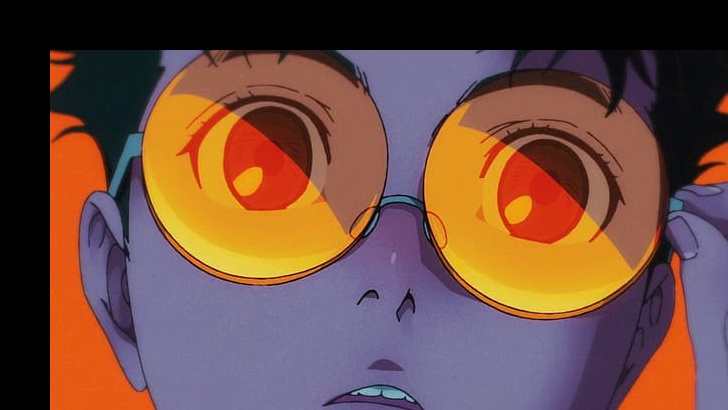
\includegraphics[width=\textwidth]{transformations/translated.jpg}
    \caption{Translation}
  \end{subfigure}
  \hfill
  \begin{subfigure}[b]{0.45\textwidth}
    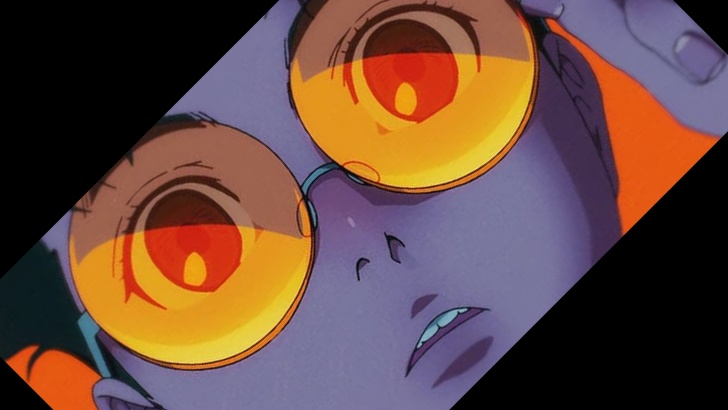
\includegraphics[width=\textwidth]{transformations/rotated.jpg}
    \caption{Rotation}
  \end{subfigure}
  \vspace{1em}
  \begin{subfigure}[b]{0.45\textwidth}
    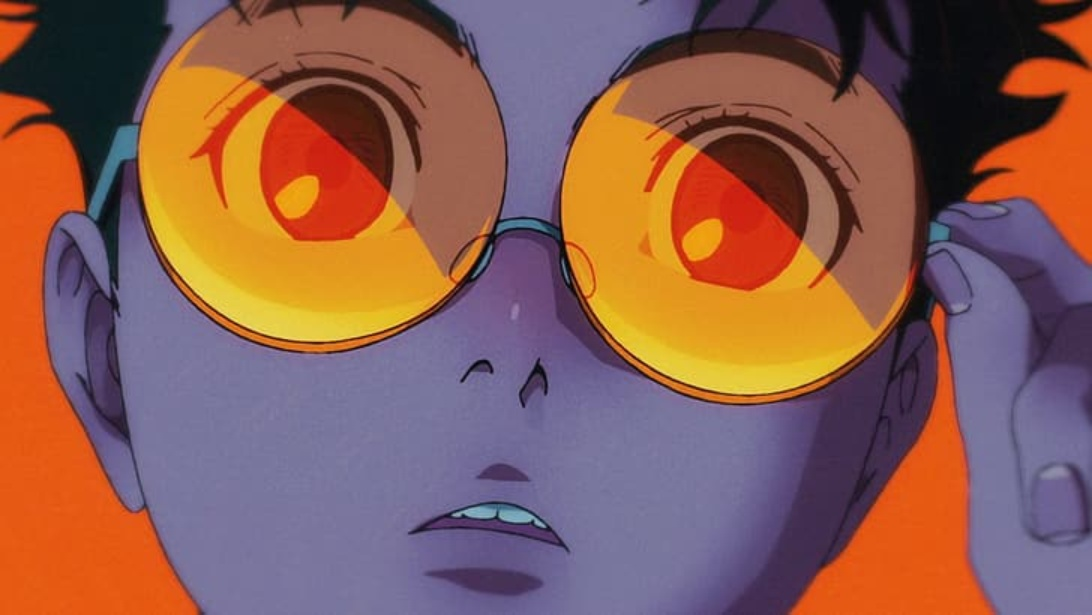
\includegraphics[width=\textwidth]{transformations/scaled.jpg}
    \caption{Scaling}
  \end{subfigure}
  \hfill
  \begin{subfigure}[b]{0.45\textwidth}
    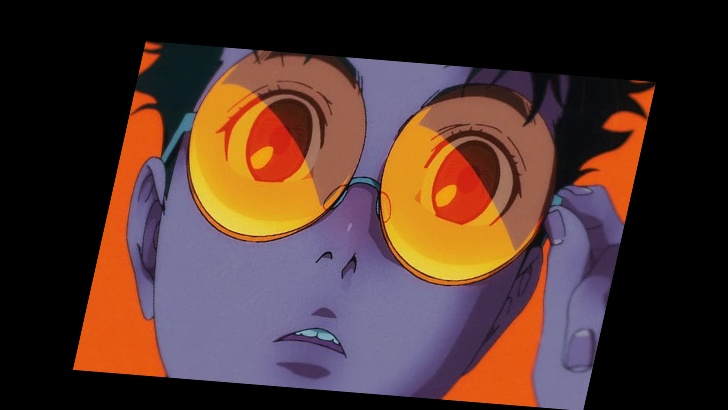
\includegraphics[width=\textwidth]{transformations/affine.jpg}
    \caption{Affine Transform}
  \end{subfigure}
  \caption{Image Transformation Results}
  \label{fig:transformations}
\end{figure}

\newpage
\section*{Experiment Number: 3}
\section{RGB to Grayscale Conversion}

\subsection{Brief Description about the Theory}
This experiment implements the luminance method for converting RGB images to grayscale using the standard formula:

\[
  Y = 0.299R + 0.587G + 0.114B
\]

These weights are based on human perception, where the green channel has the highest contribution as the human eye is most sensitive to it.

\subsection{Experimental Details}
\subsubsection{Implementation Details}
\begin{itemize}
  \item Uses a weighted sum of RGB channels.
  \item Implements the standard luminance formula.
  \item Preserves the perceptual luminance of the original image.
\end{itemize}

\subsubsection{Technical Approach}
The conversion process follows these key steps:

\begin{enumerate}
  \item \textbf{Image Loading:}
    \begin{itemize}
      \item Reads the input RGB image using OpenCV.
      \item Converts the image to \texttt{float32} for accurate computation.
    \end{itemize}

  \item \textbf{Grayscale Conversion:}
    \begin{itemize}
      \item Applies the luminance formula: \(Y = 0.299R + 0.587G + 0.114B\).
      \item These weights ensure an accurate grayscale representation.
      \item Red channel contributes 29.9\%.
      \item Green channel contributes 58.7\% (humans are most sensitive to green).
      \item Blue channel contributes 11.4\%.
    \end{itemize}

  \item \textbf{Output Processing:}
    \begin{itemize}
      \item Converts the result back to \texttt{uint8} format.
      \item Saves the processed grayscale image.
    \end{itemize}
\end{enumerate}

\subsection{Results and Inferences}
The grayscale conversion successfully preserves the perceptual brightness of the original image. The resulting image maintains visual details while reducing computational complexity for further processing.

\begin{figure}[H]
  \centering
  \begin{subfigure}[b]{0.8\textwidth}
    \centering
    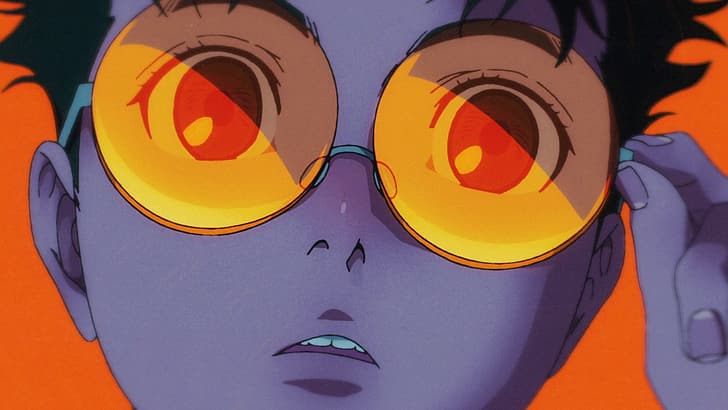
\includegraphics[width=\textwidth]{grayscale/grayscale_custom.png}
    \caption{Input RGB Image}
  \end{subfigure}
  \vspace{1em}
  \begin{subfigure}[b]{0.8\textwidth}
    \centering
    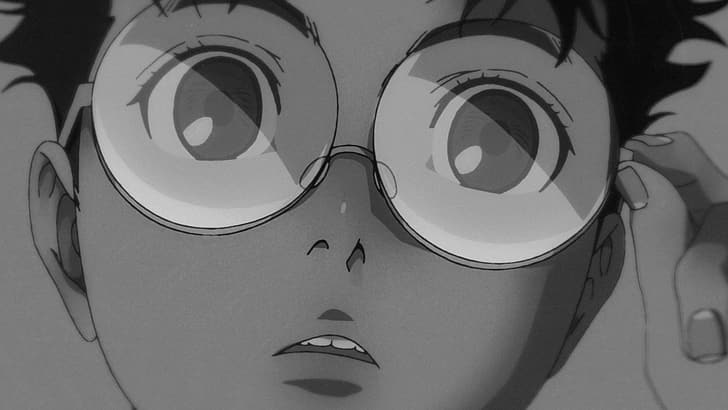
\includegraphics[width=\textwidth]{grayscale/grayscale_opencv.jpg}
    \caption{Output Grayscale Image}
  \end{subfigure}
  \caption{RGB to Grayscale Conversion Results}
  \label{fig:rgb_to_gray}
\end{figure}

\newpage
\section*{Experiment Number: 4}
\section{Intensity Resolution Reduction}

\subsection{Brief Description about the Theory}
Intensity resolution refers to the number of distinct intensity levels that an image can represent. Standard grayscale images use 8-bit representation, allowing 256 levels of intensity (0-255). Reducing the bit depth decreases the number of available intensity levels, leading to visual effects such as posterization and loss of smooth gradients.

\subsection{Experimental Details}
\subsubsection{Intensity Levels and Bit Depth}
\begin{itemize}
  \item \textbf{8-bit:} 256 levels (0-255)
  \item \textbf{7-bit:} 128 levels (0-127)
  \item \textbf{6-bit:} 64 levels (0-63)
  \item \textbf{5-bit:} 32 levels (0-31)
  \item \textbf{4-bit:} 16 levels (0-15)
  \item \textbf{3-bit:} 8 levels (0-7)
  \item \textbf{2-bit:} 4 levels (0-3)
\end{itemize}

\subsubsection{Implementation Details}
The bit depth reduction process consists of the following steps:

\begin{enumerate}
  \item \textbf{Calculate Scale Factor:}
    The scale factor for a given bit depth is computed as:
    \[
      scale = \frac{255}{2^{bits} - 1}
    \]

  \item \textbf{Quantize Pixel Values:}
    The pixel intensity values are adjusted based on the reduced bit depth:
    \[
      I_{reduced} = \lfloor \frac{I_{original}}{scale} \rfloor \times scale
    \]

  \item \textbf{Visual Effects:}
    \begin{itemize}
      \item Reduced number of intensity levels.
      \item Possible posterization effects.
      \item Loss of fine intensity gradients.
    \end{itemize}
\end{enumerate}

\subsection{Results and Inferences}
The experiment successfully demonstrated the effects of reducing intensity resolution. As the bit depth decreases, the image loses fine details, leading to visible intensity banding and posterization effects. Lower bit depths significantly impact image quality, which is crucial for applications involving image compression and display optimizations.

\begin{figure}[H]
  \centering
  \begin{subfigure}[b]{0.8\textwidth}
    \centering
    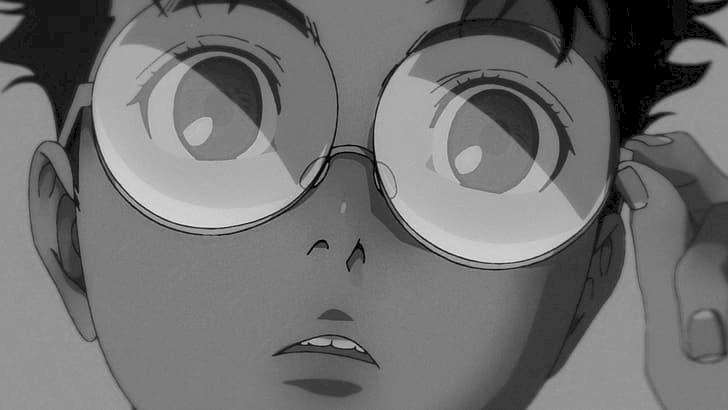
\includegraphics[width=\textwidth]{intensity/reduced_8bit.jpg}
    \caption{Input Grayscale Image}
  \end{subfigure}
  \vspace{1em}
  \begin{subfigure}[b]{0.8\textwidth}
    \centering
    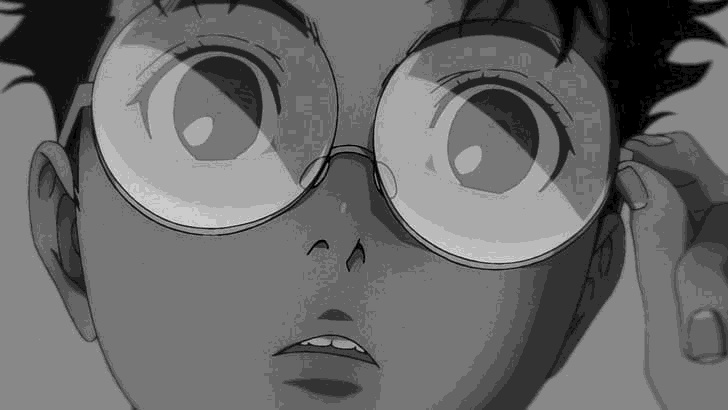
\includegraphics[width=\textwidth]{intensity/reduced_4bit.jpg}
    \caption{Output Image with Reduced Intensity Resolution}
  \end{subfigure}
  \caption{Intensity Resolution Reduction Results}
  \label{fig:intensity_resolution}
\end{figure}

\newpage
\section*{Experiment Number: 5}
\section{Spatial Resolution Modification}

\subsection{Brief Description about the Theory}
Spatial resolution refers to the number of pixels used to represent an image. Higher resolution images contain more detail but require more storage, while lower resolution images lose detail but reduce file size. This experiment investigates the impact of resolution changes through downsampling and upsampling techniques.

\subsection{Experimental Details}
\subsubsection{Resolution Levels and Effects}
\begin{itemize}
  \item \textbf{Higher resolution:} More detail, larger file size.
  \item \textbf{Lower resolution:} Less detail, smaller file size.
  \item \textbf{Common resolutions tested:} 256×256, 128×128, 64×64.
\end{itemize}

\subsubsection{Implementation Details}
The process of modifying spatial resolution involves:

\begin{enumerate}
  \item \textbf{Downsampling:}
    \begin{itemize}
      \item Reduce image dimensions by integer factors.
      \item Apply an anti-aliasing filter before resizing to minimize artifacts.
      \item Preserve aspect ratio to avoid distortion.
    \end{itemize}

  \item \textbf{Quality Assessment:}
    \begin{itemize}
      \item Visual comparison of detail retention across different resolutions.
      \item Analysis of information loss due to resolution reduction.
      \item Comparison of storage size for different resolutions.
    \end{itemize}
\end{enumerate}

\subsection{Results and Inferences}
The experiment demonstrated that reducing spatial resolution leads to loss of detail and increased pixelation. Lower-resolution images retain overall structure but exhibit a noticeable decrease in fine details. The trade-off between resolution and storage size is crucial in applications such as image compression and transmission.

\begin{figure}[H]
  \centering
  \begin{subfigure}[b]{\textwidth}
    \centering
    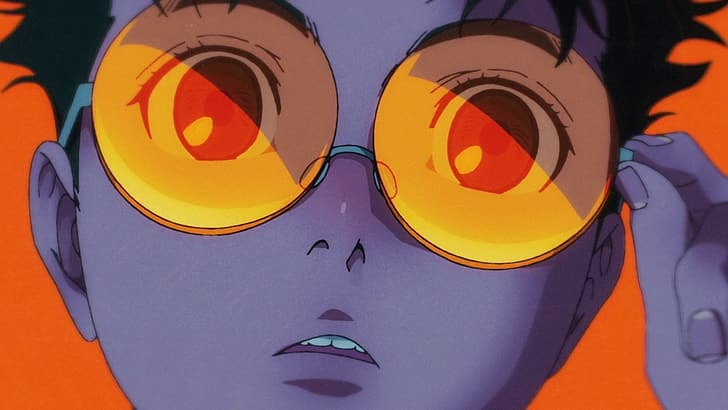
\includegraphics[width=0.8\textwidth]{spatial/spatial_reduced_100percent.jpg}
    \caption{Input Image}
  \end{subfigure}

  \vspace{2em}

  \begin{subfigure}[b]{0.32\textwidth}
    \centering
    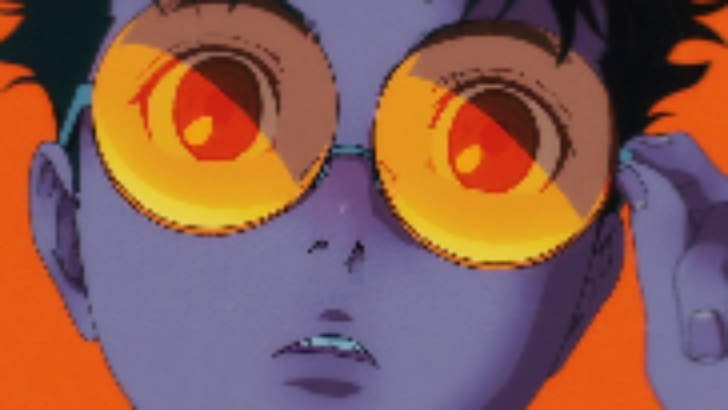
\includegraphics[width=\textwidth]{spatial/spatial_reduced_25percent.jpg}
    \caption{Output Image 64×64}
  \end{subfigure}
  \hfill
  \begin{subfigure}[b]{0.32\textwidth}
    \centering
    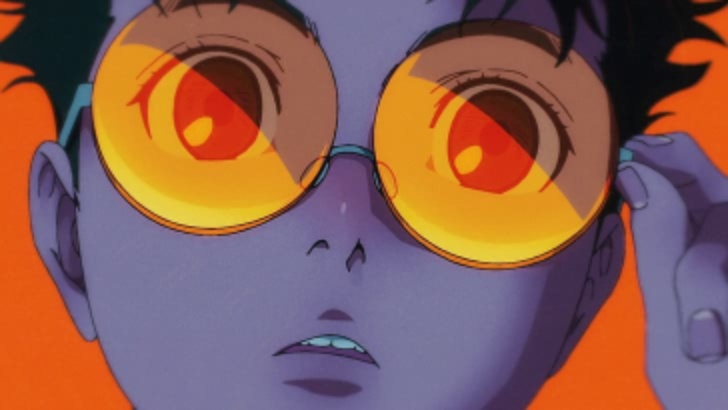
\includegraphics[width=\textwidth]{spatial/spatial_reduced_50percent.jpg}
    \caption{Output Image 128×128}
  \end{subfigure}
  \hfill
  \begin{subfigure}[b]{0.32\textwidth}
    \centering
    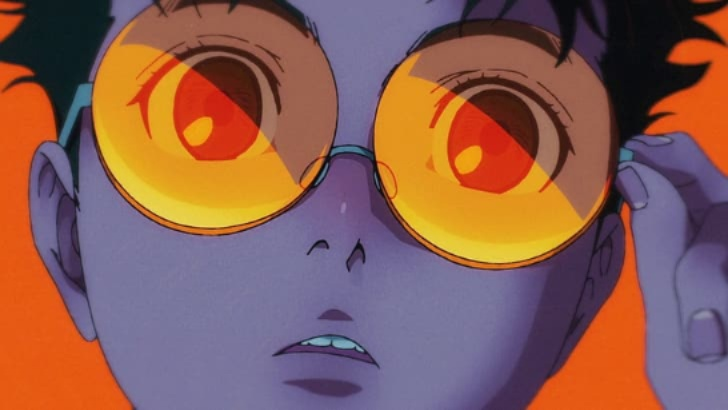
\includegraphics[width=\textwidth]{spatial/spatial_reduced_75percent.jpg}
    \caption{Output Image 256×256}
  \end{subfigure}
  \caption{Spatial Resolution Variation Results}
  \label{fig:spatial_resolution}
\end{figure}

\newpage
\section*{Experiment Number: 6}
\section{Interpolation Techniques for Image Resizing}

\subsection{Brief Description about the Theory}
Interpolation is a fundamental technique in image processing used for resizing and reconstructing images. It estimates pixel values based on neighboring pixels, ensuring smoother transformations when scaling images. Different interpolation methods offer varying trade-offs between speed and quality.

\subsection{Experimental Details}
\subsubsection{Types of Interpolation}
\begin{itemize}
  \item \textbf{Nearest Neighbor:}
    \begin{itemize}
      \item Simplest method that assigns the value of the nearest pixel.
      \item Formula: \( f(x,y) = f(\text{round}(x), \text{round}(y)) \).
      \item Fastest but produces blocky and jagged edges.
    \end{itemize}

  \item \textbf{Bilinear Interpolation:}
    \begin{itemize}
      \item Performs linear interpolation in both horizontal and vertical directions.
      \item Uses a \(2 \times 2\) neighborhood.
      \item Provides smoother results compared to nearest neighbor.
      \item Formula involves weighted averaging of four nearest pixels.
    \end{itemize}

  \item \textbf{Bicubic Interpolation:}
    \begin{itemize}
      \item Uses cubic interpolation in both directions.
      \item Considers a \(4 \times 4\) neighborhood, utilizing 16 surrounding pixels.
      \item Produces the highest quality results, preserving fine details and reducing artifacts.
      \item More computationally expensive than bilinear interpolation.
    \end{itemize}
\end{itemize}

\subsubsection{Implementation Comparison}
\begin{itemize}
  \item \textbf{Quality vs. Computation Time:}
    \begin{itemize}
      \item Nearest Neighbor: Fastest but lowest quality.
      \item Bilinear: Balanced trade-off between speed and quality.
      \item Bicubic: Highest quality but computationally expensive.
    \end{itemize}

  \item \textbf{Use Cases:}
    \begin{itemize}
      \item Nearest Neighbor: Pixel art, binary images, and discrete labeling.
      \item Bilinear: Real-time applications where moderate quality is acceptable.
      \item Bicubic: High-quality resizing for photography, printing, and medical imaging.
    \end{itemize}
\end{itemize}

\subsection{Results and Inferences}
The experiment demonstrated that nearest neighbor interpolation is fast but results in visible pixelation, while bilinear interpolation improves smoothness but may blur fine details. Bicubic interpolation provides the highest visual quality, making it ideal for detailed images but requires more computation.

\begin{figure}[H]
  \centering
  \begin{subfigure}[b]{0.45\textwidth}
    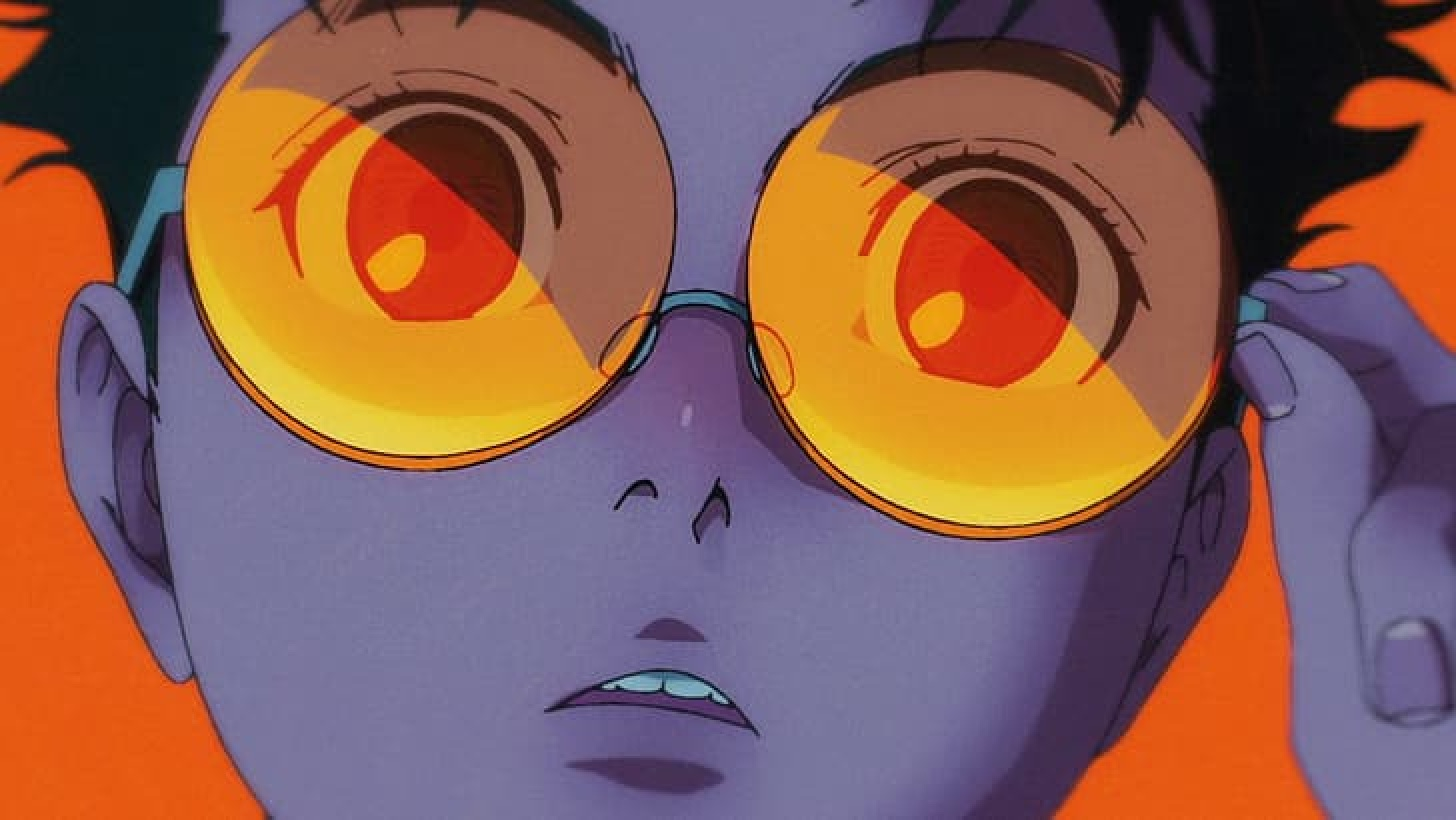
\includegraphics[width=\textwidth]{interpolation/interpolation_nearest_2x.jpg}
    \caption{Nearest Neighbor (2x)}
  \end{subfigure}
  \hfill
  \begin{subfigure}[b]{0.45\textwidth}
    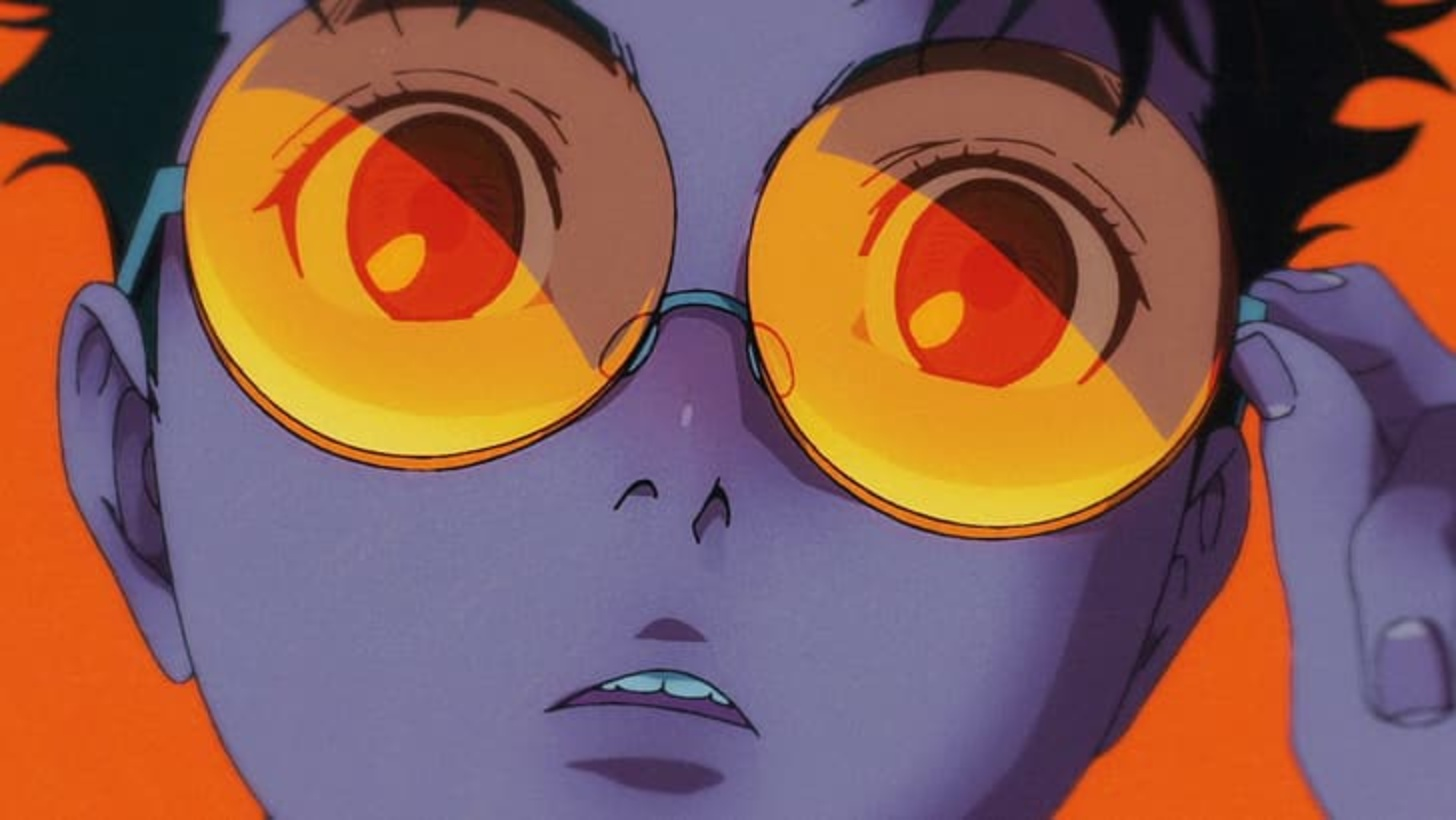
\includegraphics[width=\textwidth]{interpolation/interpolation_bilinear_2x.jpg}
    \caption{Bilinear (2x)}
  \end{subfigure}
  \vspace{1em}
  \begin{subfigure}[b]{0.45\textwidth}
    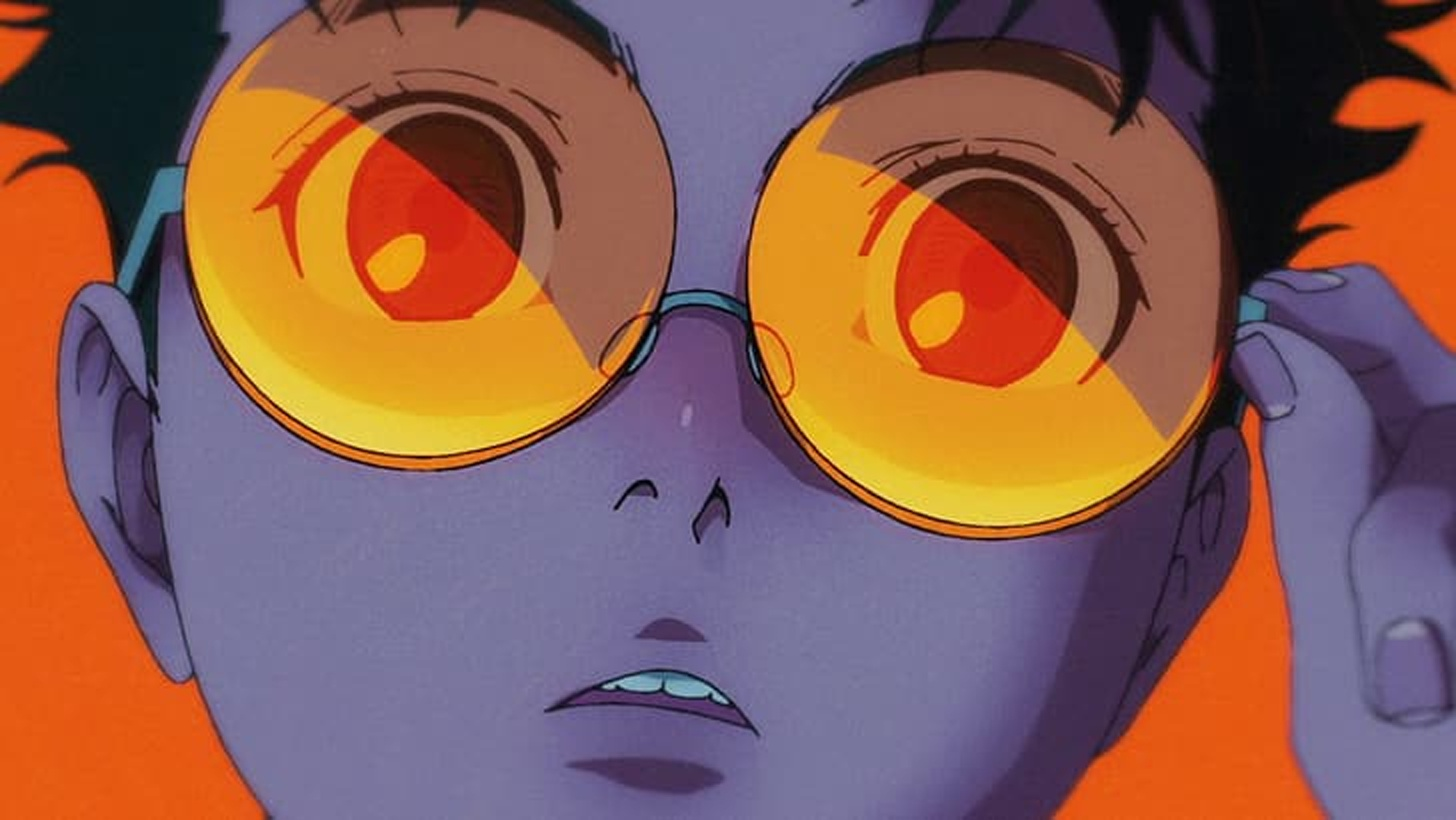
\includegraphics[width=\textwidth]{interpolation/interpolation_bicubic_2x.jpg}
    \caption{Bicubic (2x)}
  \end{subfigure}
  \hfill
  \begin{subfigure}[b]{0.45\textwidth}
    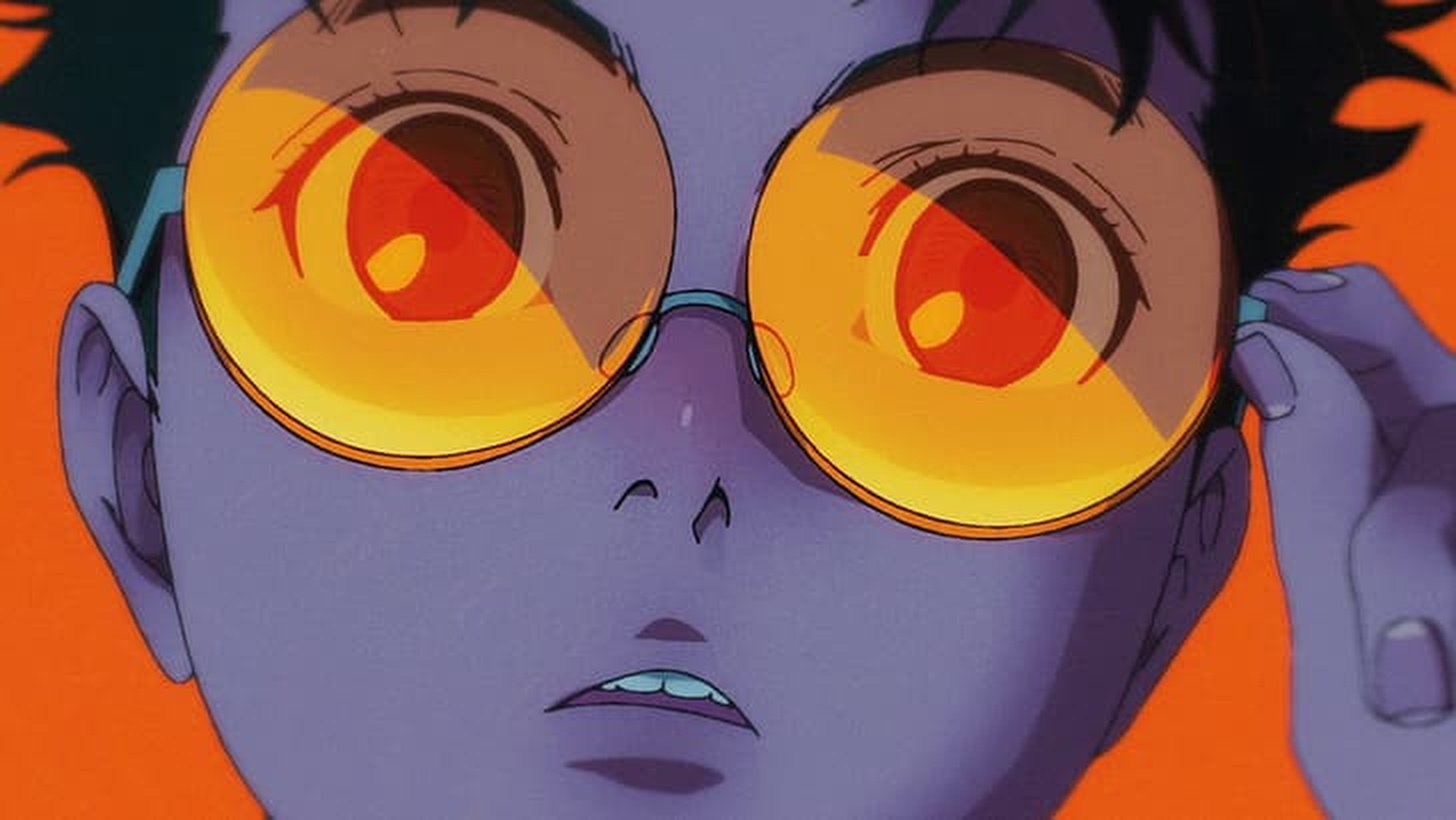
\includegraphics[width=\textwidth]{interpolation/interpolation_lanczos_2x.jpg}
    \caption{Lanczos (2x)}
  \end{subfigure}
  \caption{Interpolation Results}
  \label{fig:interpolation}
\end{figure}

\newpage
\section*{Experiment Number: 7}
\section{Image Blurring for Smoothing and Noise Reduction}

\subsection{Brief Description about the Theory}
Image blurring is a fundamental technique used in image processing to reduce noise, smooth textures, and simulate realistic depth effects. Different blurring methods apply varying kernel operations to achieve distinct smoothing effects.

\subsection{Experimental Details}
\subsubsection{Implemented Blurring Techniques}

\begin{itemize}
  \item \textbf{Gaussian Blur:}
    \begin{itemize}
      \item Uses a Gaussian kernel for weighted averaging.
      \item Kernel size: \(15 \times 15\) pixels.
      \item Implements the 2D Gaussian function:
        \[
          G(x,y) = \frac{1}{2\pi\sigma^2}e^{-\frac{x^2+y^2}{2\sigma^2}}
        \]
      \item Effective for noise reduction while preserving edges.
    \end{itemize}

  \item \textbf{Box Filter (Average Blur):}
    \begin{itemize}
      \item Computes the average of all pixels in the kernel window.
      \item Each pixel contributes equally to the result.
      \item Fastest method but less effective for high-frequency noise.
    \end{itemize}

  \item \textbf{Motion Blur:}
    \begin{itemize}
      \item Simulates the effect of motion in an image.
      \item Uses a directional kernel to create streaks in a specific direction.
      \item The intensity and angle of blur can be controlled.
    \end{itemize}

  \item \textbf{Focus Blur:}
    \begin{itemize}
      \item Simulates a depth-of-field effect similar to real camera focus.
      \item Applies varying blur intensities based on a depth map.
      \item Useful for creating realistic depth effects in images.
    \end{itemize}
\end{itemize}

\subsection{Results and Inferences}
The experiment demonstrated that Gaussian Blur is highly effective for noise reduction while maintaining edge structures. The Box Filter produces uniform blurring but lacks adaptability for noise suppression. Motion Blur effectively simulates real-world motion effects, while Focus Blur mimics realistic depth perception.

\begin{figure}[H]
  \centering
  \begin{subfigure}[b]{0.45\textwidth}
    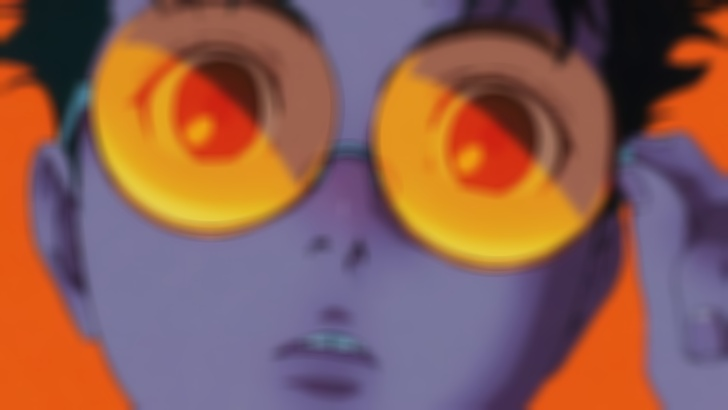
\includegraphics[width=\textwidth]{blurring/box_blur_15x15.jpg}
    \caption{Box Filter Result}
  \end{subfigure}
  \hfill
  \begin{subfigure}[b]{0.45\textwidth}
    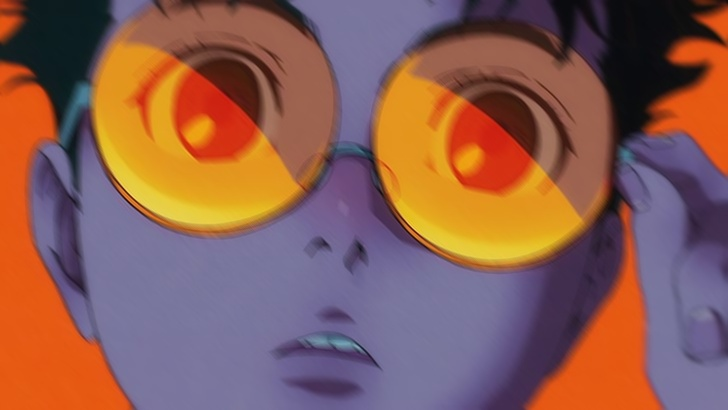
\includegraphics[width=\textwidth]{blurring/motion_blur_45deg.jpg}
    \caption{Motion Blur Result}
  \end{subfigure}
  \vspace{1em}
  \begin{subfigure}[b]{0.45\textwidth}
    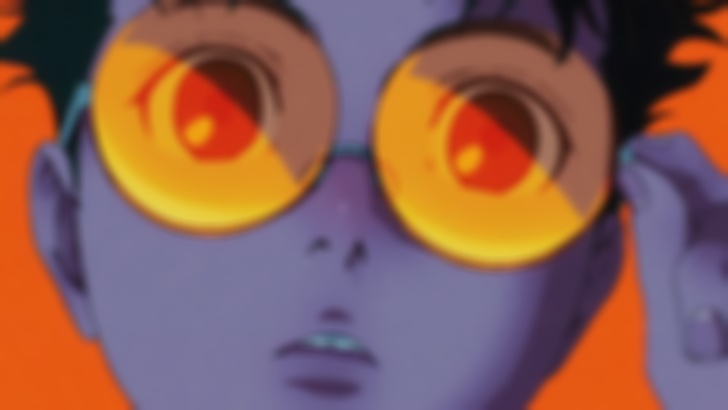
\includegraphics[width=\textwidth]{blurring/gaussian_blur_15x15.jpg}
    \caption{Gaussian Blur Input}
  \end{subfigure}
  \hfill
  \begin{subfigure}[b]{0.45\textwidth}
    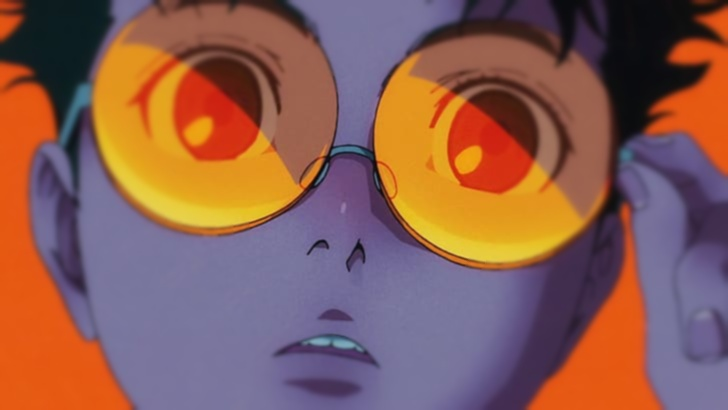
\includegraphics[width=\textwidth]{blurring/focus_blur_r100.jpg}
    \caption{Focus Blur Output}
  \end{subfigure}
  \caption{Image Blurring Results}
  \label{fig:blurring}
\end{figure}

\newpage
\section*{Experiment Number: 8}
\section{Histogram Processing for Image Enhancement}

\subsection{Brief Description about the Theory}
Histogram processing is a crucial technique in image enhancement and analysis. It helps improve contrast, brightness, and overall visibility of details in an image. The histogram represents the frequency distribution of pixel intensities, allowing for transformations like histogram equalization and histogram matching.

\subsection{Experimental Details}
\subsubsection{Implemented Techniques}

\begin{itemize}
  \item \textbf{Histogram Equalization:}
    \begin{itemize}
      \item Redistributes intensity values to enhance contrast.
      \item Uses the cumulative distribution function (CDF) for transformation.
      \item Particularly useful for images with poor contrast.
    \end{itemize}

  \item \textbf{Histogram Matching:}
    \begin{itemize}
      \item Adjusts the histogram of one image to match that of another.
      \item Ensures similar brightness and contrast levels between images.
      \item Uses a lookup table (LUT) for pixel intensity mapping.
    \end{itemize}
\end{itemize}

\subsubsection{Mathematical Foundation}
\begin{itemize}
  \item \textbf{Cumulative Distribution Function (CDF):}
    \[
      CDF(i) = \sum_{j=0}^{i} \frac{histogram(j)}{total\_pixels}
    \]
  \item \textbf{Lookup Table Generation for Matching:}
    \[
      LUT[i] = \arg\min_j |CDF_{target}(j) - CDF_{source}(i)|
    \]
\end{itemize}

\subsection{Implementation Details}
\subsubsection{Histogram Equalization}
\begin{enumerate}
  \item Compute the histogram of the input image.
  \item Calculate the cumulative distribution function (CDF).
  \item Normalize and use CDF to remap intensity values.
  \item Generate the enhanced output image.
\end{enumerate}

\subsubsection{Histogram Matching}
\begin{enumerate}
  \item Convert both source and target images to grayscale.
  \item Compute histograms and cumulative distribution functions (CDFs).
  \item Generate a mapping function using a lookup table (LUT).
  \item Apply the mapping to the source image to match the target histogram.
\end{enumerate}

\subsection{Results and Inferences}
Histogram equalization successfully improves contrast by spreading intensity values across the full dynamic range. Histogram matching allows controlled modification of image brightness and contrast, making it useful for image normalization tasks.

\begin{figure}[H]
  \centering
  \begin{subfigure}[b]{0.8\textwidth}
    \centering
    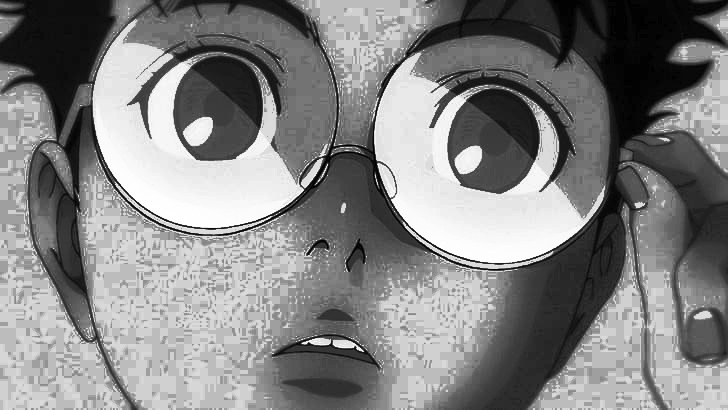
\includegraphics[width=\textwidth]{histogram/histogram_equalized.jpg}
    \caption{Histogram Equalization Result}
  \end{subfigure}
  \vspace{1em}
  \begin{subfigure}[b]{0.8\textwidth}
    \centering
    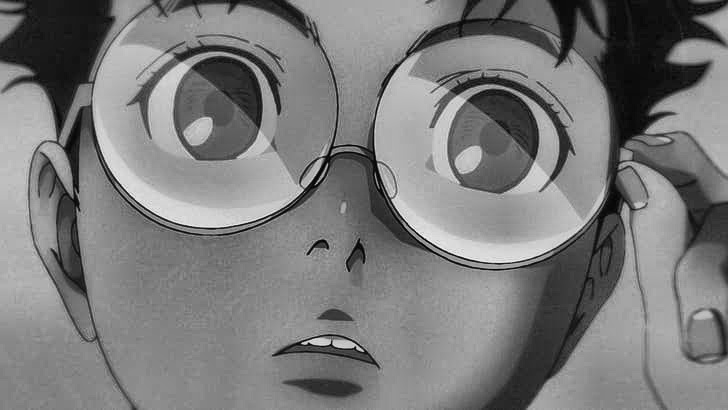
\includegraphics[width=\textwidth]{histogram/adaptive_hist_clip2_grid8x8.jpg}
    \caption{Adaptive Histogram Equalization Result}
  \end{subfigure}
  \caption{Histogram Processing Results}
  \label{fig:histogram}
\end{figure}

\newpage
\section*{Experiment Number: 9}
\section{Frequency Domain Filtering with Box Filter}

\subsection{Brief Description about the Theory}
Frequency domain filtering is a powerful technique in image processing where transformations are performed in the frequency domain rather than the spatial domain. The Box filter, a simple low-pass filter, is applied in the frequency domain to remove high-frequency components, effectively smoothing the image.

\subsection{Experimental Details}
\subsubsection{Implemented Approach}
\begin{itemize}
  \item A Box filter is used to attenuate high-frequency components.
  \item Both the image and the filter are transformed to the frequency domain using Fast Fourier Transform (FFT).
  \item Filtering is performed by element-wise multiplication in the frequency domain.
  \item The processed image is then transformed back to the spatial domain using the Inverse FFT.
\end{itemize}

\subsection{Technical Approach}
The filtering process follows these key steps:

\subsubsection{Image Loading}
\begin{itemize}
  \item The input image is read and converted to grayscale if necessary.
  \item The image is converted to \texttt{float32} for precise FFT computation.
\end{itemize}

\subsubsection{Box Filter Creation}
\begin{itemize}
  \item A Box filter of size \(50 \times 50\) is created in the spatial domain.
  \item The filter is padded to match the dimensions of the input image.
\end{itemize}

\subsubsection{Frequency Domain Filtering}
\begin{itemize}
  \item The image and the Box filter are both transformed to the frequency domain using FFT.
  \item The frequency domain representations of the filter and the image are multiplied element-wise.
  \item The inverse FFT is applied to convert the filtered image back to the spatial domain.
\end{itemize}

\subsubsection{Output Processing}
\begin{itemize}
  \item The resulting image is displayed and saved for analysis.
\end{itemize}

\subsection{Results and Inferences}
Applying the Box filter in the frequency domain effectively removes high-frequency noise and results in a smoother image. The method demonstrates how frequency domain filtering can provide efficient noise reduction and low-pass filtering.

\begin{figure}[H]
  \centering
  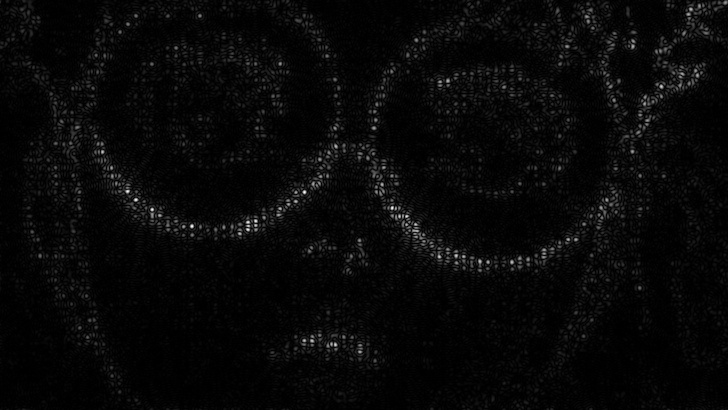
\includegraphics[width=0.8\textwidth]{freq_box/box_filtered.jpg}
  \caption{Frequency Domain Filtering with Box Filter}
  \label{fig:box_filter}
\end{figure}

\newpage
\section*{Experiment Number: 10}
\section{Frequency Domain Filtering with Gaussian Filter}

\subsection{Brief Description about the Theory}
Frequency domain filtering is an essential technique in image processing that modifies image frequencies to enhance or suppress specific details. The Gaussian filter is a low-pass filter that smoothly attenuates high-frequency components, preserving essential image structures while reducing noise.

\subsection{Experimental Details}
\subsubsection{Implemented Approach}
\begin{itemize}
  \item A Gaussian filter is designed to suppress high-frequency noise while retaining low-frequency details.
  \item The image and filter are transformed into the frequency domain using the Fast Fourier Transform (FFT).
  \item Filtering is performed through element-wise multiplication in the frequency domain.
  \item The processed image is reconstructed via the Inverse FFT.
\end{itemize}

\subsection{Technical Approach}
The filtering process follows these key steps:

\subsubsection{Image Loading}
\begin{itemize}
  \item The input image is read and converted to grayscale if necessary.
  \item The image is converted to \texttt{float32} format for precise FFT computation.
\end{itemize}

\subsubsection{Gaussian Filter Creation}
\begin{itemize}
  \item A Gaussian filter is created in the spatial domain using the standard Gaussian function:
    \[
      G(x,y) = \frac{1}{2\pi\sigma^2}e^{-\frac{x^2+y^2}{2\sigma^2}}
    \]
  \item The filter is padded to match the dimensions of the input image.
\end{itemize}

\subsubsection{Frequency Domain Filtering}
\begin{itemize}
  \item The image and the Gaussian filter are transformed into the frequency domain using FFT.
  \item The frequency representations of the filter and the image are multiplied element-wise.
  \item The inverse FFT is applied to reconstruct the filtered image in the spatial domain.
\end{itemize}

\subsubsection{Output Processing}
\begin{itemize}
  \item The final processed image is displayed and saved for further analysis.
\end{itemize}

\subsection{Results and Inferences}
Applying the Gaussian filter in the frequency domain effectively reduces noise while maintaining smooth transitions. This method is widely used in applications like denoising, image enhancement, and edge-preserving smoothing.

\begin{figure}[H]
  \centering
  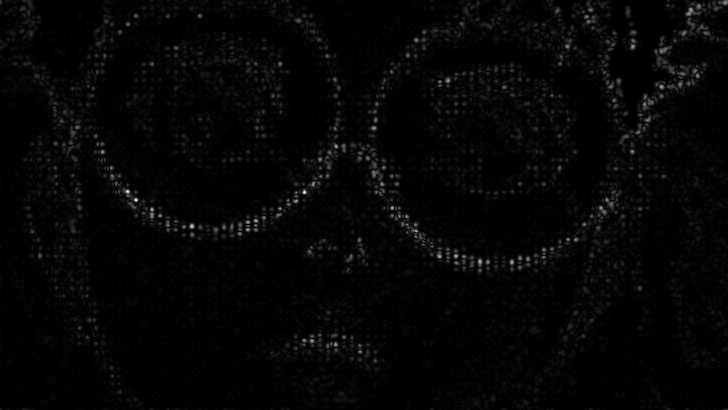
\includegraphics[width=0.8\textwidth]{freq_gaussian/gaussian_filtered_sigma10.jpg}
  \caption{Frequency Domain Filtering with Gaussian Filter}
  \label{fig:gauss_filter}
\end{figure}

\newpage
\section*{Experiment Number: 11}
\section{Frequency Domain Filtering with Random Filter}

\subsection{Brief Description about the Theory}
Frequency domain filtering is a technique that processes an image by modifying its frequency components. Unlike standard filters (e.g., Gaussian or Box filters), a random filter applies an arbitrary transformation, which can introduce unpredictable alterations to the image structure.

\subsection{Experimental Details}
\subsubsection{Implemented Approach}
\begin{itemize}
  \item A random filter is generated using a uniform distribution of random values.
  \item The random filter is created in the spatial domain and then transformed into the frequency domain using FFT.
  \item Image filtering is performed by multiplying the frequency representation of the image with that of the random filter.
\end{itemize}

\subsection{Technical Approach}
The filtering process consists of the following steps:

\subsubsection{Image Loading}
\begin{itemize}
  \item The input image is read and converted to grayscale if required.
  \item The image is converted to \texttt{float32} format to maintain numerical precision during FFT computations.
\end{itemize}

\subsubsection{Random Filter Creation}
\begin{itemize}
  \item A random filter is generated with uniform random values across the image dimensions.
  \item Unlike traditional filters, this filter lacks predefined characteristics and introduces unpredictable transformations.
\end{itemize}

\subsubsection{Frequency Domain Filtering}
\begin{itemize}
  \item The random filter and the input image are transformed into the frequency domain using FFT.
  \item Element-wise multiplication is performed between the frequency representations of the image and the random filter.
  \item The result is transformed back to the spatial domain using the inverse FFT (IFFT).
\end{itemize}

\subsubsection{Output Processing}
\begin{itemize}
  \item The final filtered image is displayed and saved for analysis.
\end{itemize}

\subsection{Results and Inferences}
Applying a random filter in the frequency domain results in unpredictable modifications to the image. The effects can vary from subtle changes in texture to complete distortion, making this method more suitable for artistic transformations or experimental processing rather than structured image enhancement.

\begin{figure}[H]
  \centering
  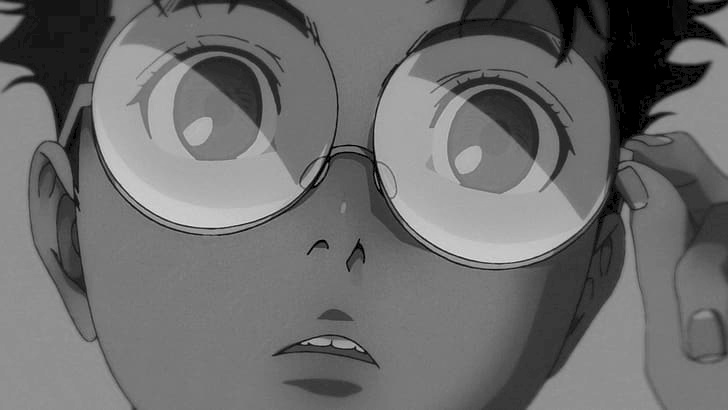
\includegraphics[width=0.8\textwidth]{freq_random/random_filtered_d50_s10.jpg}
  \caption{Frequency Domain Filtering with Random Filter}
  \label{fig:random_filter}
\end{figure}

\newpage
\section*{Experiment Number: 12}
\section{Finding DCT of a Sequence}

\subsection{Brief Description about the Theory}
The Discrete Cosine Transform (DCT) is a widely used mathematical transformation in signal processing, particularly in image compression techniques like JPEG. It transforms a sequence from the time domain into the frequency domain, helping in energy compaction and reducing redundancy.

\subsection{Experimental Details}
\subsubsection{Implemented Approach}
\begin{itemize}
  \item Compute the DCT of a given sequence using SciPy's \texttt{fft.dct} function.
  \item Modify the DCT coefficients by setting the last element to zero.
  \item Apply the Inverse DCT (IDCT) using \texttt{fft.idct} to reconstruct the modified sequence.
  \item Compare the original and reconstructed sequences.
\end{itemize}

\subsection{Technical Approach}
The experiment follows these key steps:

\subsubsection{DCT Computation}
\begin{itemize}
  \item The input sequence is transformed into the frequency domain using the Discrete Cosine Transform.
  \item The DCT coefficients represent frequency components, with lower indices capturing low-frequency content and higher indices capturing finer details.
\end{itemize}

\subsubsection{Coefficient Modification}
\begin{itemize}
  \item The last DCT coefficient is set to zero.
  \item This step demonstrates how removing high-frequency components affects the reconstruction.
\end{itemize}

\subsubsection{IDCT Reconstruction}
\begin{itemize}
  \item The modified DCT coefficients are transformed back into the time domain using the Inverse Discrete Cosine Transform (IDCT).
  \item The resulting sequence is compared with the original sequence to observe the impact of removing the last coefficient.
\end{itemize}

\subsection{Results and Inferences}
Removing the last DCT coefficient slightly alters the reconstructed sequence but generally retains the overall structure. This experiment demonstrates the effect of modifying frequency components and their impact on data representation.

\begin{figure}[H]
  \centering
  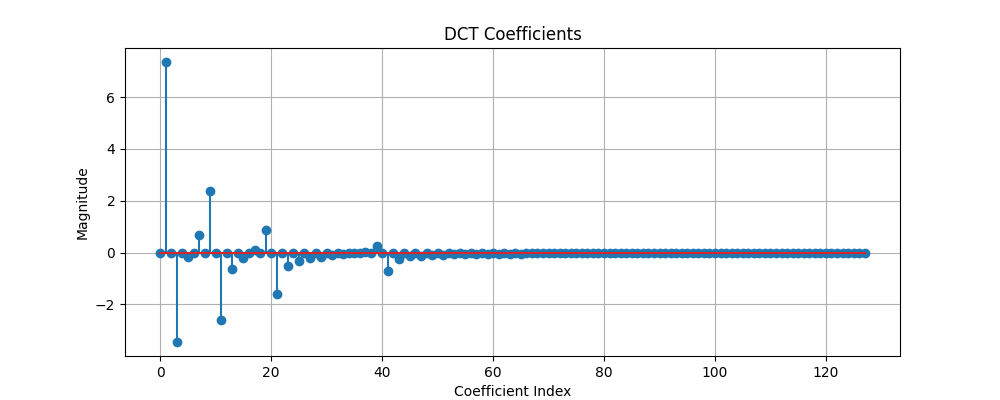
\includegraphics[width=0.7\textwidth]{dct/dct_coefficients.png}
  \caption{DCT Experiment Results}
  \label{fig:finddct}
\end{figure}

\newpage
\section*{Experiment Number: 13}
\section{Sequence Energy Compaction}

\subsection{Brief Description about the Theory}
The Discrete Cosine Transform (DCT) is widely used for energy compaction, concentrating most of a signal's energy into a few coefficients. This property is essential in compression techniques such as JPEG, where low-energy components can be discarded with minimal loss in quality. This experiment evaluates how energy is distributed in the original sequence and its DCT representation, including the effect of setting the last DCT coefficient to zero.

\subsection{Experimental Details}
\subsubsection{Implemented Approach}
\begin{itemize}
  \item Compute the total energy of the original sequence.
  \item Perform the Discrete Cosine Transform (DCT) on the sequence.
  \item Calculate the energy of the DCT coefficients.
  \item Modify the DCT representation by setting the last coefficient to zero.
  \item Compute the energy of the modified DCT sequence and compare it with the original.
\end{itemize}

\subsection{Technical Approach}
The experiment follows these key steps:

\subsubsection{Energy Computation}
\begin{itemize}
  \item The total energy of a sequence is computed as:
    \[
      E_{\text{sequence}} = \sum_{i=0}^{N-1} x[i]^2
    \]
    where \( x[i] \) represents the sequence values.
\end{itemize}

\subsubsection{DCT Energy Distribution}
\begin{itemize}
  \item The energy of the DCT-transformed sequence is calculated similarly.
  \item This transformation helps visualize how energy is concentrated in specific coefficients.
\end{itemize}

\subsubsection{Effect of Coefficient Modification}
\begin{itemize}
  \item The last DCT coefficient is set to zero.
  \item The resulting energy is recalculated to observe any loss.
\end{itemize}

\subsection{Results and Inferences}
This experiment demonstrates that the DCT effectively compacts energy into fewer coefficients, and modifying a single coefficient has a minimal but noticeable effect on total energy.

\begin{figure}[H]
  \centering
  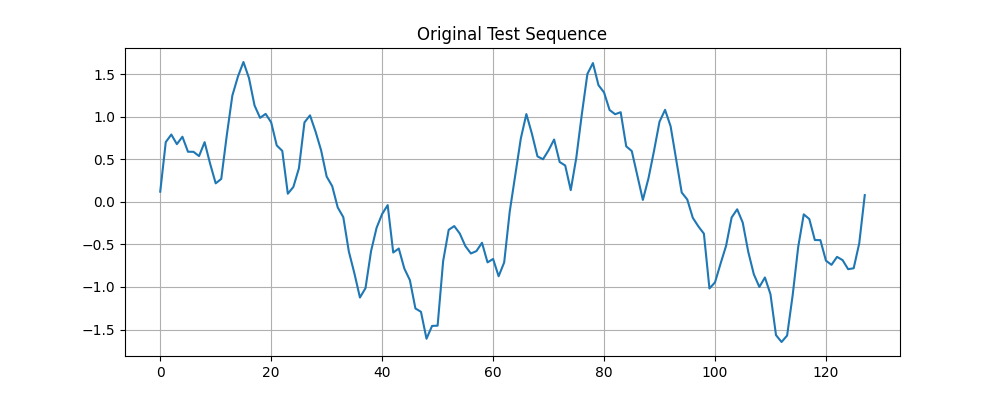
\includegraphics[width=0.7\textwidth]{sequence_energy/sequence_energy.png}
  \caption{Sequence Energy Experiment Results}
  \label{fig:seqenergy}
\end{figure}

\newpage
\section*{Experiment Number: 14}
\section{Image Energy Compaction}

\subsection{Brief Description about the Theory}
Energy compaction is a fundamental principle in image processing and compression. The Discrete Cosine Transform (DCT) helps concentrate image energy into fewer coefficients, enabling efficient compression. By retaining only significant coefficients, we can reconstruct an image with minimal perceptual loss.

\subsection{Experimental Details}
\subsubsection{Implemented Approach}
\begin{itemize}
  \item Compute the 2D Discrete Cosine Transform (DCT) of an image.
  \item Retain only 50\% of the DCT coefficients (low-frequency components).
  \item Apply the Inverse DCT (IDCT) to reconstruct the image.
  \item Compare the original, DCT, and reconstructed images.
\end{itemize}

\subsection{Technical Approach}
The experiment follows these key steps:

\subsubsection{2D DCT Computation}
\begin{itemize}
  \item The input image is transformed into the frequency domain using the 2D DCT.
  \item This transformation expresses the image as a sum of frequency components.
  \item The DCT coefficients are analyzed for energy distribution.
\end{itemize}

\subsubsection{Coefficient Cutoff}
\begin{itemize}
  \item Only the lower 50\% of frequencies (high-energy components) are retained.
  \item The remaining coefficients are set to zero to simulate compression.
\end{itemize}

\subsubsection{Image Reconstruction via IDCT}
\begin{itemize}
  \item The truncated DCT coefficients are used to reconstruct the image via IDCT.
  \item The reconstructed image is compared against the original.
\end{itemize}

\subsection{Results and Inferences}
This experiment demonstrates that a significant portion of an image's energy is concentrated in lower frequencies. Even after removing 50\% of the coefficients, the reconstructed image retains most of the visual information, illustrating the effectiveness of energy compaction in compression.

\begin{figure}[H]
  \centering
  \begin{subfigure}[b]{0.7\textwidth}
    \centering
    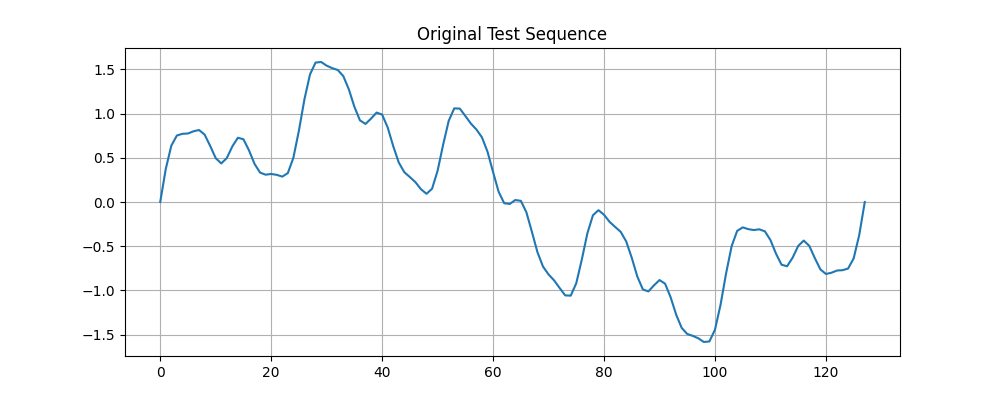
\includegraphics[width=\textwidth]{dct/original_sequence.png}
    \caption{Original Sequence}
  \end{subfigure}
  \begin{subfigure}[b]{0.7\textwidth}
    \centering
    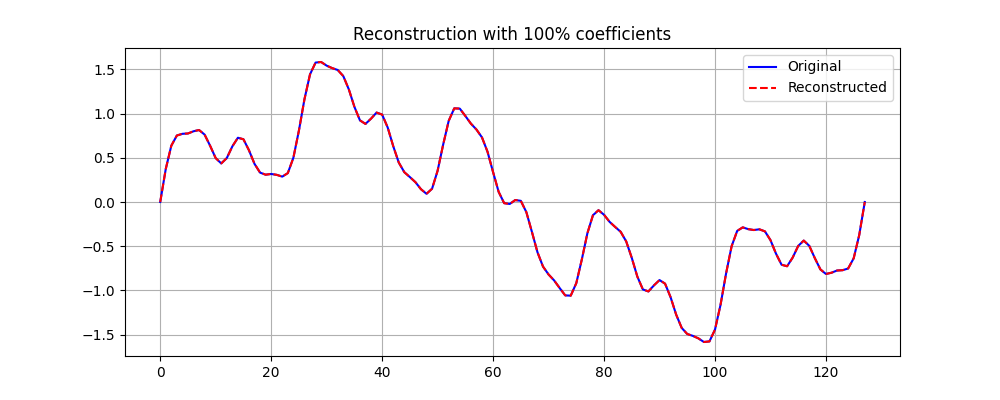
\includegraphics[width=\textwidth]{dct/reconstruction_100percent.png}
    \caption{Reconstructed Sequence}
  \end{subfigure}
  \caption{DCT Analysis Results}
  \label{fig:dct_analysis}
\end{figure}

\newpage
\section*{Experiment Number: 15}
\section{Wavelet Decomposition}

\subsection{Brief Description about the Theory}
Wavelet decomposition provides a multi-resolution analysis of images, making it a powerful tool in image compression and feature extraction. Unlike the Fourier Transform, which analyzes signals in the frequency domain, wavelets analyze images in both spatial and frequency domains, allowing localized feature representation.

\subsection{Technical Background}
Wavelet transforms break down an image into multiple frequency components at different scales:
\begin{itemize}
  \item \textbf{Haar Wavelet Decomposition}: Splits an image into four sub-bands using wavelet filters.
  \item \textbf{Frequency Components}: Produces low-frequency (\textbf{LL}) and high-frequency components (\textbf{LH}, \textbf{HL}, \textbf{HH}).
  \item \textbf{Multi-Resolution Analysis}: Helps analyze the image at different levels of detail.
\end{itemize}

\subsection{Implementation Details}
The experiment utilizes the PyWavelets library (\texttt{pywt}) for 2D wavelet decomposition:

\subsubsection{Decomposition Process}
\begin{enumerate}
  \item \textbf{Pre-processing:}
    \begin{itemize}
      \item Convert the input image to grayscale.
      \item Normalize pixel values for better numerical stability.
    \end{itemize}

  \item \textbf{Wavelet Transformation:}
    \begin{itemize}
      \item Apply Haar wavelet decomposition using \texttt{pywt.dwt2()}.
      \item Extract four sub-bands: LL (approximation), LH (horizontal details), HL (vertical details), HH (diagonal details).
    \end{itemize}

  \item \textbf{Visualization and Analysis:}
    \begin{itemize}
      \item Display and analyze the four sub-band images.
      \item Compare the original image with its wavelet decomposition.
    \end{itemize}
\end{enumerate}

\subsection{Results and Inferences}
This experiment highlights the effectiveness of Haar wavelet decomposition in representing an image's frequency components. The LL sub-band retains most of the structural information, while the LH, HL, and HH components emphasize finer details.

\begin{figure}[H]
  \centering
  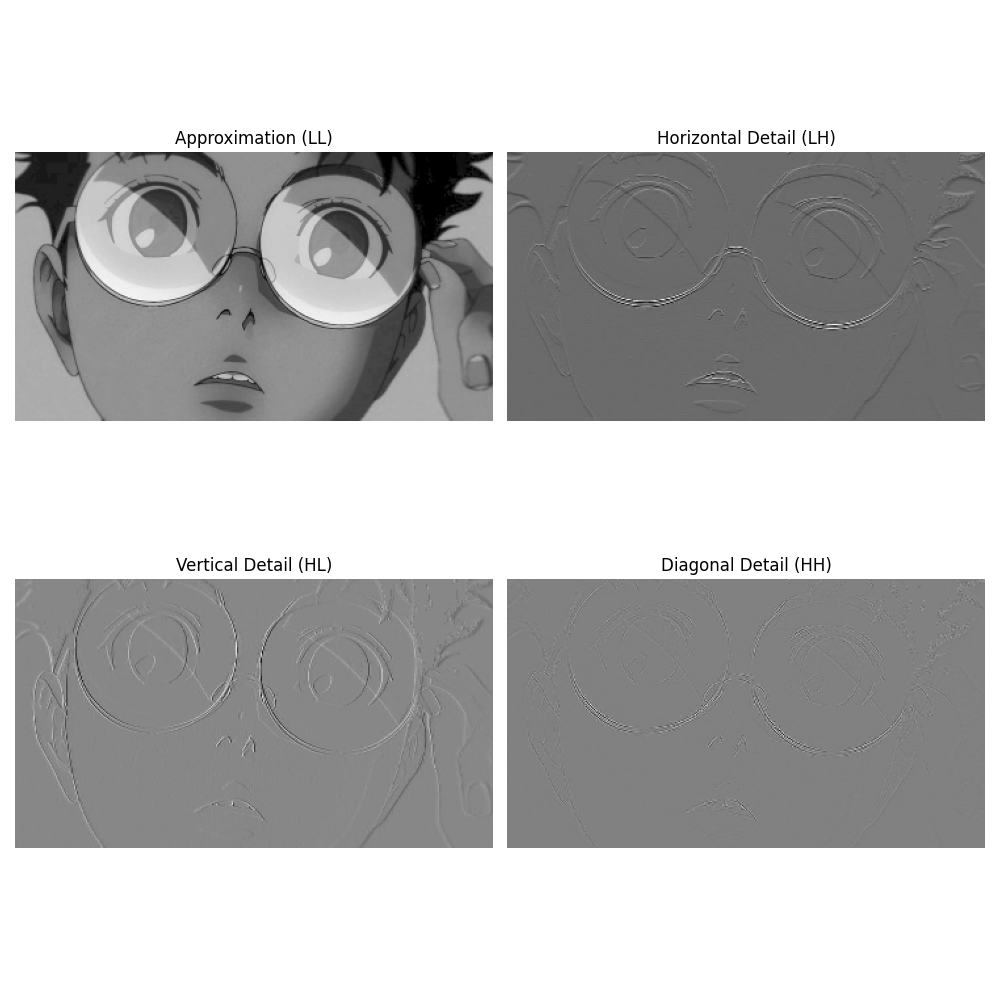
\includegraphics[width=0.8\textwidth]{wavelet/decomposition.png}
  \caption{Wavelet Experiment Results - Decomposed Sub-bands}
  \label{fig:wavelet}
\end{figure}

\newpage
\section*{Experiment Number: 16}
\section{Wavelet-Based Image Denoising}

\subsection{Brief Description about the Theory}
Wavelet-based denoising is a powerful technique for image noise reduction, leveraging the ability of wavelet transforms to separate low and high-frequency components. This experiment applies Haar wavelet decomposition to analyze and suppress noise while preserving image details.

\subsection{Technical Background}
Wavelet transforms are useful for image denoising because they allow selective modification of frequency components:
\begin{itemize}
  \item \textbf{Wavelet Decomposition:} The image is decomposed into four sub-bands:
    \begin{itemize}
      \item \textbf{LL (Approximation):} Low-frequency components (main structure of the image).
      \item \textbf{LH (Horizontal details)}, \textbf{HL (Vertical details)}, and \textbf{HH (Diagonal details)}: High-frequency components (edges and noise).
    \end{itemize}
  \item \textbf{Denoising Methods:}
    \begin{itemize}
      \item \textbf{Method 1:} All detail coefficients (\textbf{LH, HL, HH}) are set to zero.
      \item \textbf{Method 2:} Thresholding is applied to the detail coefficients, setting values below a defined threshold to zero.
    \end{itemize}
  \item \textbf{Wavelet Reconstruction:} The denoised image is reconstructed using the Inverse Discrete Wavelet Transform (IDWT).
  \item \textbf{Quality Evaluation:} Peak Signal-to-Noise Ratio (PSNR) is computed to assess denoising effectiveness.
\end{itemize}

\subsection{Implementation Details}
The experiment is implemented using:
\begin{itemize}
  \item \textbf{OpenCV:} Image loading and preprocessing.
  \item \textbf{PyWavelets (pywt):} Haar wavelet decomposition and reconstruction.
  \item \textbf{Scikit-Image:} PSNR computation for image quality evaluation.
\end{itemize}

\subsubsection{Processing Steps}
\begin{enumerate}
  \item \textbf{Image Preparation:}
    \begin{itemize}
      \item Convert the image to grayscale and resize it.
      \item Add Gaussian noise (\(\mu = 0\), \(\sigma = 25\)) to simulate a noisy environment.
    \end{itemize}

  \item \textbf{Wavelet Transformation:}
    \begin{itemize}
      \item Perform Haar wavelet decomposition using \texttt{pywt.dwt2()}.
      \item Extract the four sub-bands (\textbf{LL, LH, HL, HH}).
    \end{itemize}

  \item \textbf{Denoising Techniques:}
    \begin{itemize}
      \item Method 1: Set all LH, HL, HH coefficients to zero.
      \item Method 2: Apply thresholding to remove weak high-frequency components.
    \end{itemize}

  \item \textbf{Wavelet Reconstruction:}
    \begin{itemize}
      \item Reconstruct the image using the inverse wavelet transform.
    \end{itemize}

  \item \textbf{Quality Analysis:}
    \begin{itemize}
      \item Compute PSNR values to compare the original, noisy, and denoised images.
    \end{itemize}
\end{enumerate}

\subsection{Results and Inferences}
This experiment demonstrates that wavelet-based denoising effectively suppresses noise while preserving structural details. Method-2 (thresholding) provides a better balance between noise reduction and edge preservation, as observed in the PSNR comparison.

\begin{figure}[H]
  \centering
  \begin{subfigure}[b]{0.48\textwidth}
    \centering
    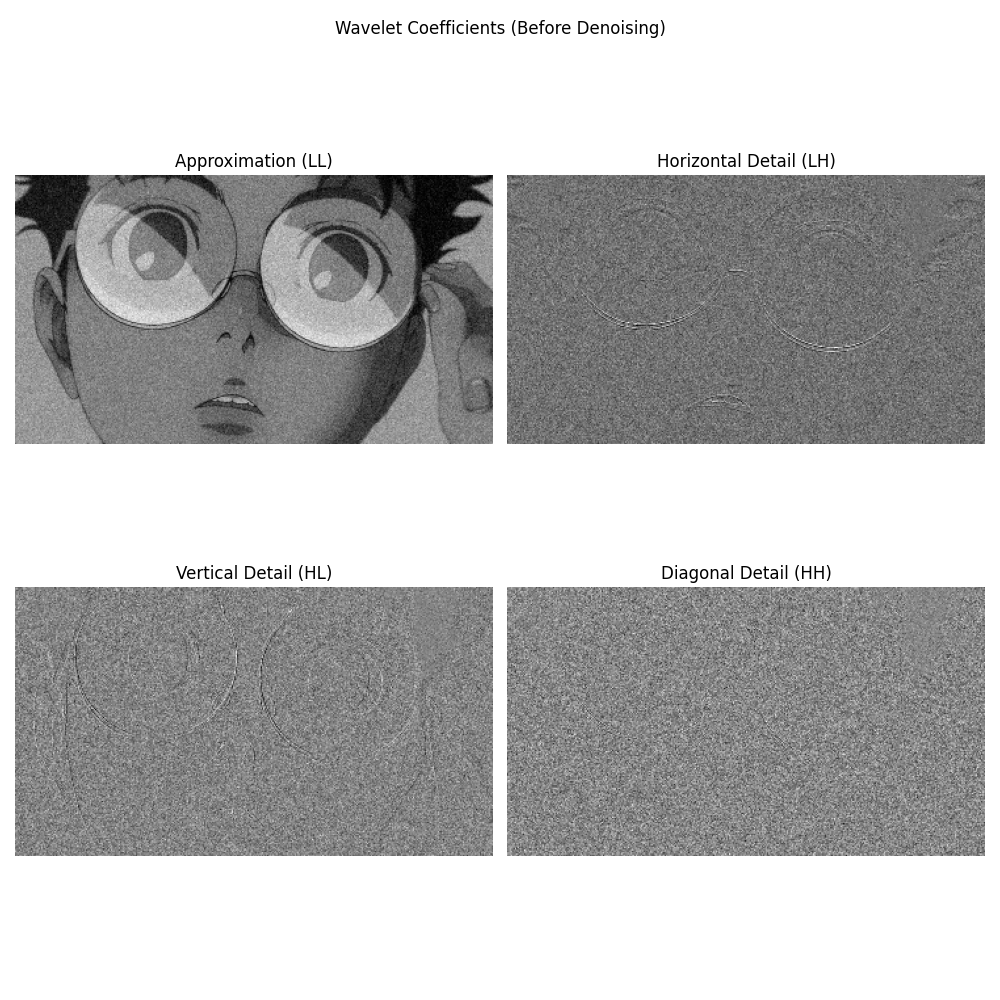
\includegraphics[width=\textwidth]{wavelet/coefficients_before.png}
    \caption{Wavelet Coefficients before Denoising}
  \end{subfigure}
  \begin{subfigure}[b]{0.48\textwidth}
    \centering
    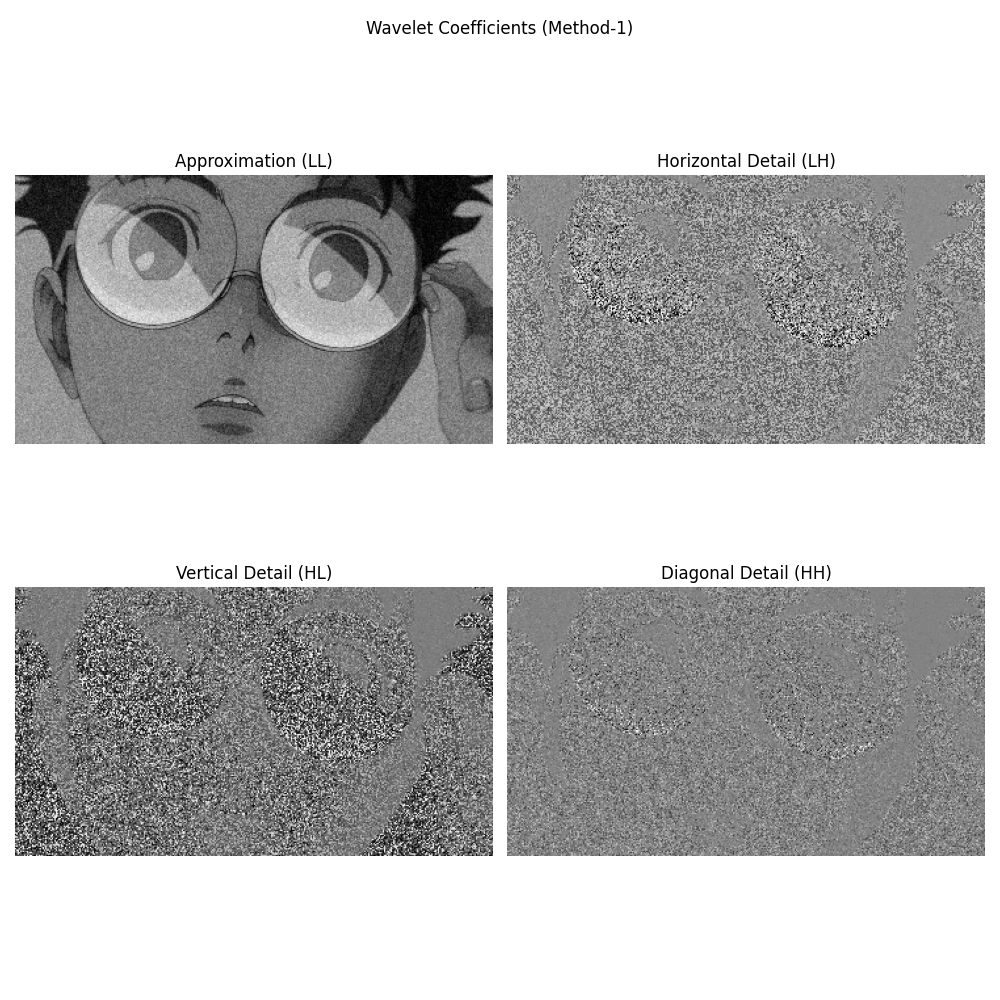
\includegraphics[width=\textwidth]{wavelet/coefficients_method1.png}
    \caption{Wavelet Coefficients after Method-1 Denoising}
  \end{subfigure}
  \begin{subfigure}[b]{0.48\textwidth}
    \centering
    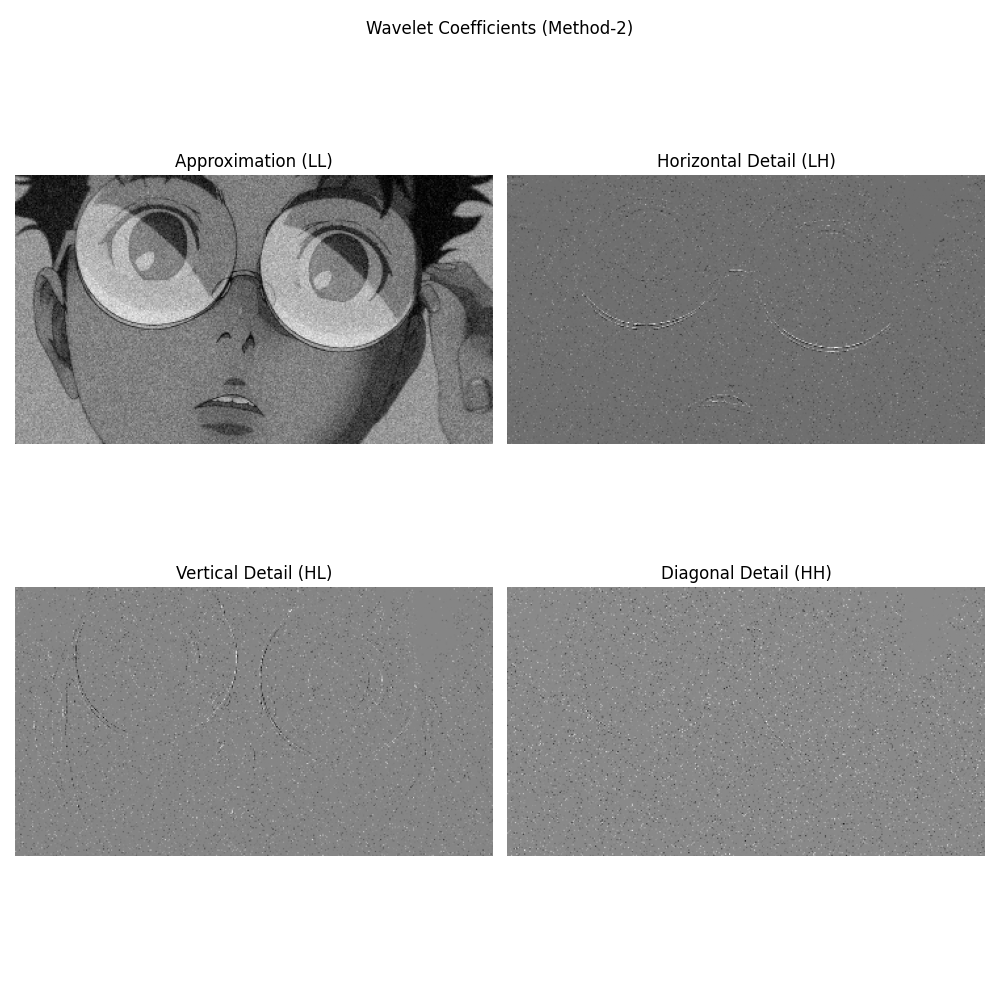
\includegraphics[width=\textwidth]{wavelet/coefficients_method2.png}
    \caption{Wavelet Coefficients after Method-2 Denoising}
  \end{subfigure}
  \begin{subfigure}[b]{0.48\textwidth}
    \centering
    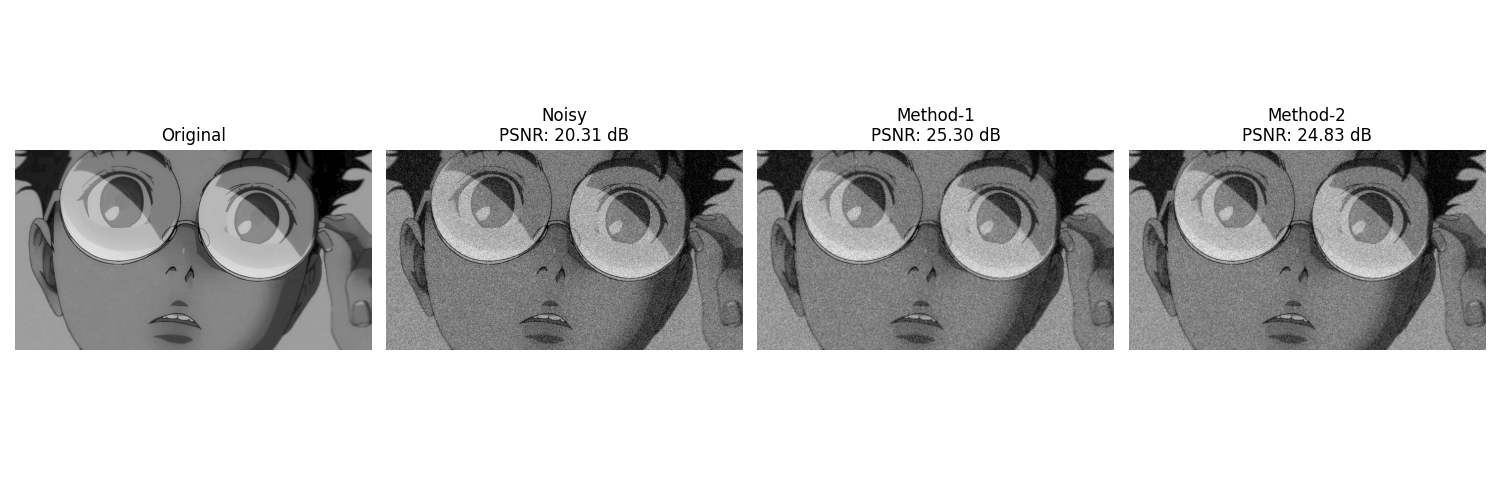
\includegraphics[width=\textwidth]{wavelet/denoised_comparison.png}
    \caption{Original vs. Denoised Image}
  \end{subfigure}
  \begin{subfigure}[b]{0.48\textwidth}
    \centering
    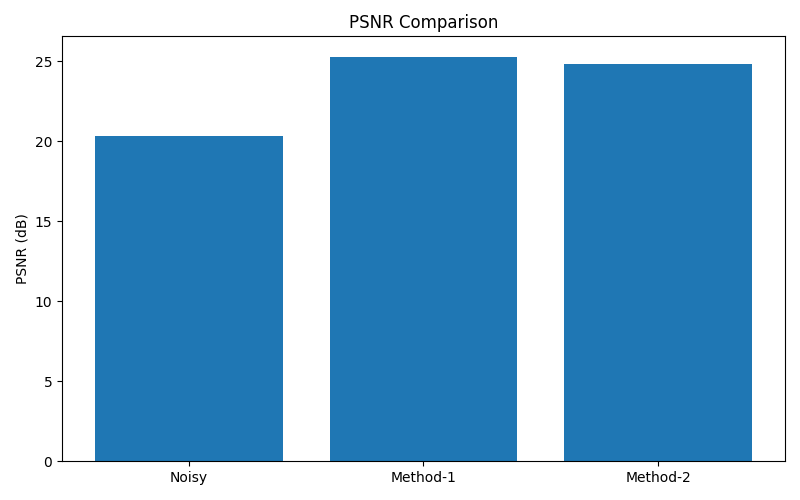
\includegraphics[width=\textwidth]{wavelet/psnr_comparison.png}
    \caption{PSNR Comparison of Different Methods}
  \end{subfigure}
  \caption{Wavelet-Based Image Denoising Results}
  \label{fig:wavelet_denoising}
\end{figure}

\end{document}